% Name: Fundamental polygons
% Description: Squares whose edges are glued in the direction of their arrows to make the sphere, the torus, the Klein bottle, and the real projective plane.
% Tags: fundamental polygon, torus, Klein bottle, projective plane, surfaces

\usetikzlibrary{arrows.meta, decorations.markings}

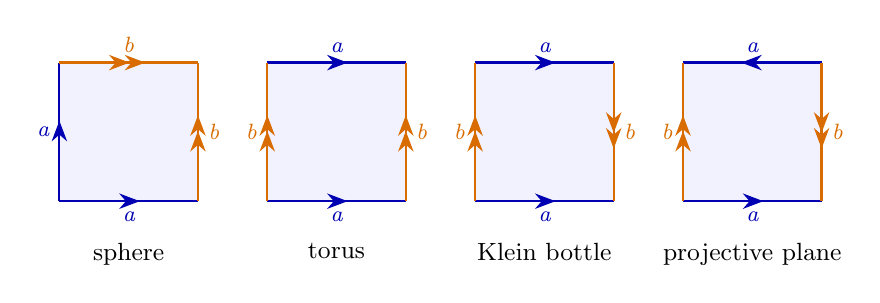
\begin{tikzpicture}[scale=0.88, thick, every node/.style={font=\small},
    a/.style={blue!70!black, postaction={decorate}, decoration={markings, mark=at position 0.58 with {\arrow{Stealth[length=2.6mm]}}}},
    b/.style={orange!85!black, postaction={decorate}, decoration={markings, mark=at position 0.62 with {\arrow{Stealth[length=2.6mm]}\arrow[xshift=-2mm]{Stealth[length=2.6mm]}}}},
    lab/.style={font=\footnotesize\itshape}]
  % Each edge's path runs the way its arrow points: single arrows are glued to single, double to double
  \foreach \x/\name in {0/sphere, 3/torus, 6/Klein bottle, 9/projective plane} {
    \fill[blue!5] (\x,0) rectangle ++(2,2);
    \node[below=4mm] at (\x+1,0) {\name};
  }
  \draw[a] (0,0) -- node[lab, below] {a} (2,0);   \draw[a] (0,0) -- node[lab, left] {a} (0,2);
  \draw[b] (0,2) -- node[lab, above] {b} (2,2);   \draw[b] (2,0) -- node[lab, right] {b} (2,2);
  \draw[a] (3,0) -- node[lab, below] {a} (5,0);   \draw[a] (3,2) -- node[lab, above] {a} (5,2);
  \draw[b] (3,0) -- node[lab, left] {b} (3,2);    \draw[b] (5,0) -- node[lab, right] {b} (5,2);
  \draw[a] (6,0) -- node[lab, below] {a} (8,0);   \draw[a] (6,2) -- node[lab, above] {a} (8,2);
  \draw[b] (6,0) -- node[lab, left] {b} (6,2);    \draw[b] (8,2) -- node[lab, right] {b} (8,0);
  \draw[a] (9,0) -- node[lab, below] {a} (11,0);  \draw[a] (11,2) -- node[lab, above] {a} (9,2);
  \draw[b] (9,0) -- node[lab, left] {b} (9,2);    \draw[b] (11,2) -- node[lab, right] {b} (11,0);
\end{tikzpicture}
